\usetikzlibrary{arrows.meta,decorations.pathreplacing,shapes.misc}

\begin{frame}{splitting messages: try 1}
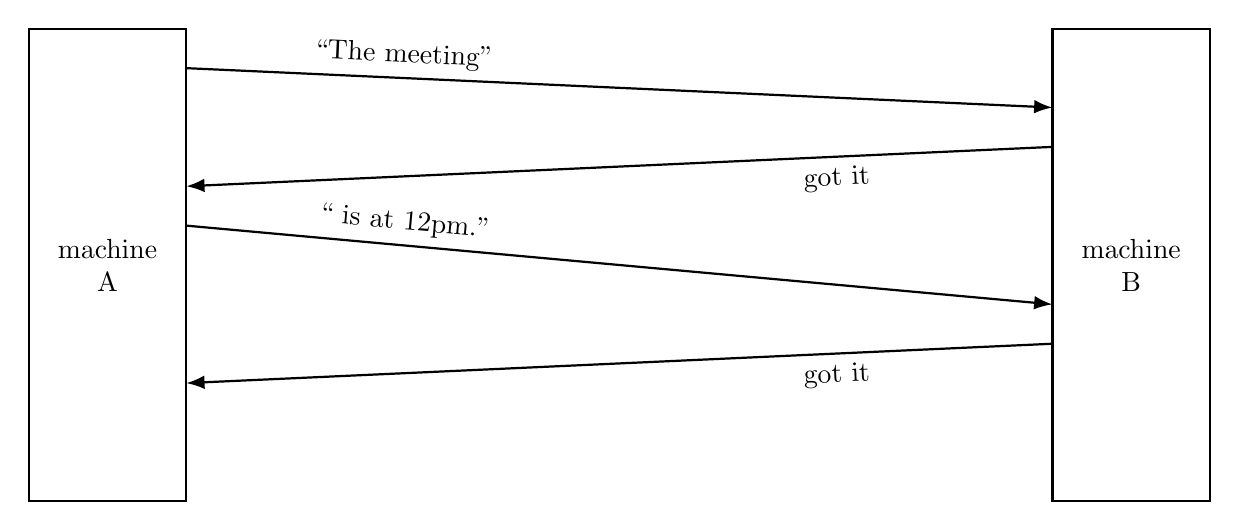
\begin{tikzpicture}
\tikzset{
    box/.style={thick},
    message/.style={draw,thick,-Latex},
    failure/.style={draw,ultra thick,red,cross out,minimum width=1cm,minimum height=1cm},
}
\begin{scope}
\draw[box] (0, 0) rectangle ++(2, -6) 
    node[midway,align=center] {machine\\A};
\draw[box] (13, 0) rectangle ++(2, -6) 
    node[midway,align=center] {machine\\B};
\draw[message] (2, -0.5) -- (13, -1) node[pos=0.25, above, sloped] {``The meeting''};
\draw[message] (13, -1.5) -- (2, -2) node[pos=0.25, sloped,below] {got it};
\draw[message] (2, -2.5) -- (13, -3.5) node[pos=0.25, above, sloped] {`` is at 12pm.''};
\draw[message] (13, -4) -- (2, -4.5) node[pos=0.25, sloped,below] {got it};
\end{scope}
\end{tikzpicture}
reconstructed message: \\
The meeting is at 12pm.
\end{frame}

\begin{frame}{splitting messages: try 1 --- problem 1}
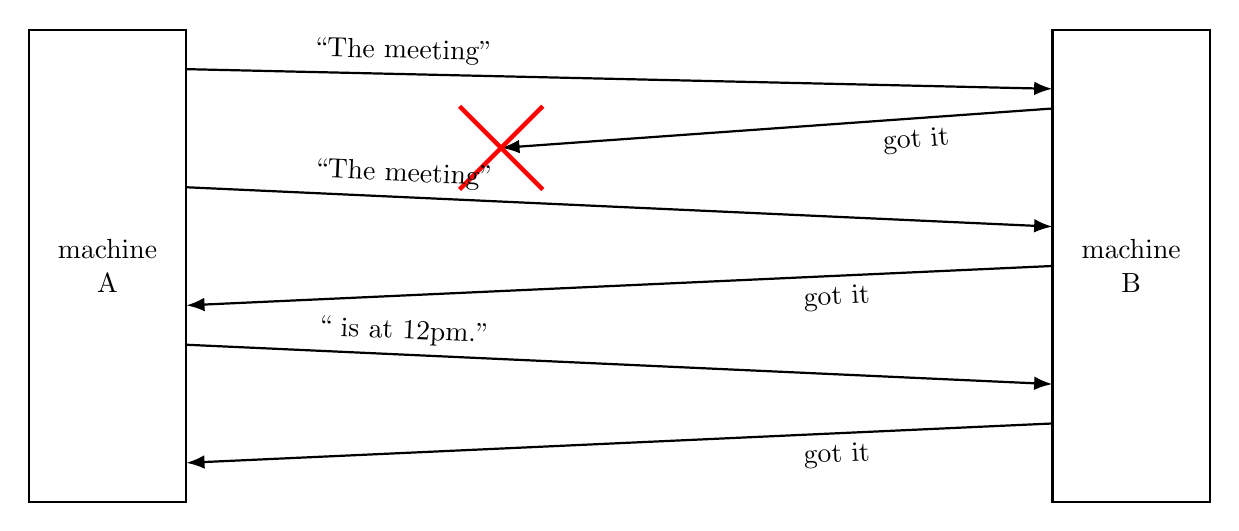
\begin{tikzpicture}
\tikzset{
    box/.style={thick},
    message/.style={draw,thick,-Latex},
    failure/.style={draw,ultra thick,red,cross out,minimum width=1cm,minimum height=1cm},
}
\begin{scope}
\draw[box] (0, 0) rectangle ++(2, -6) 
    node[midway,align=center] {machine\\A};
\draw[box] (13, 0) rectangle ++(2, -6) 
    node[midway,align=center] {machine\\B};
\draw[message] (2, -0.5) -- (13, -0.75) node[pos=0.25, above, sloped] {``The meeting''};
\draw[message] (13, -1) -- (6, -1.5) node[pos=0.25, sloped,below] {got it} node[failure] {};
\draw[message] (2, -2) -- (13, -2.5) node[pos=0.25, above, sloped] {``The meeting''};
\draw[message] (13, -3) -- (2, -3.5) node[pos=0.25, sloped,below] {got it};
\draw[message] (2, -4) -- (13, -4.5) node[pos=0.25, above, sloped] {`` is at 12pm.''};
\draw[message] (13, -5) -- (2, -5.5) node[pos=0.25, sloped,below] {got it};
\end{scope}
\end{tikzpicture}
\begin{visibleenv}<2->
reconstructed message: \\
The meetingThe meeting is at 12pm.
\end{visibleenv}
\end{frame}

\begin{frame}{exercise: other problems?}
\begin{itemize}
\item other scenarios where we'd also have problems?
\end{itemize}
\begin{tabular}{ll}
A. & message (instead of acknowledgment) is lost \\
B. & first message from A is delayed a long time by network \\
C. & acknowledgment of second message lost instead of first \\
\end{tabular}
\end{frame}

\begin{frame}{splitting messages: try 2}
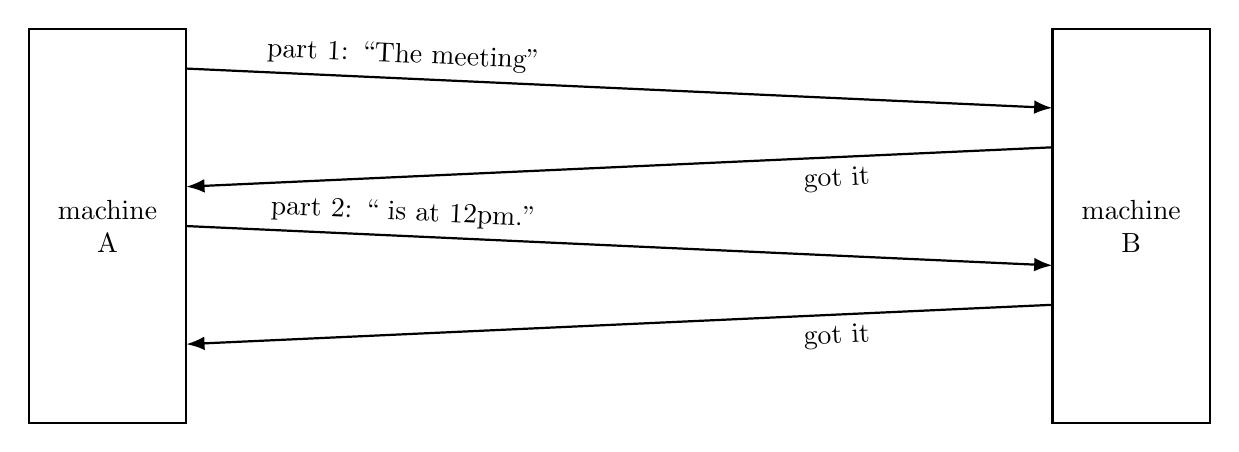
\begin{tikzpicture}
\tikzset{
    box/.style={thick},
    message/.style={draw,thick,-Latex},
    failure/.style={draw,ultra thick,red,cross out,minimum width=1cm,minimum height=1cm},
}
\begin{scope}
\draw[box] (0, 0) rectangle ++(2, -5) 
    node[midway,align=center] {machine\\A};
\draw[box] (13, 0) rectangle ++(2, -5) 
    node[midway,align=center] {machine\\B};
\draw[message] (2, -0.5) -- (13, -1) node[pos=0.25, above, sloped] {part 1: ``The meeting''};
\draw[message] (13, -1.5) -- (2, -2) node[pos=0.25, sloped,below] {got it};
\draw[message] (2, -2.5) -- (13, -3) node[pos=0.25, above, sloped] {part 2: `` is at 12pm.''};
\draw[message] (13, -3.5) -- (2, -4) node[pos=0.25, sloped,below] {got it};
\end{scope}
\end{tikzpicture}
reconstructed message: \\
The meeting is at 12pm.
\end{frame}

\begin{frame}{splitting messages: try 2 --- missed ack}
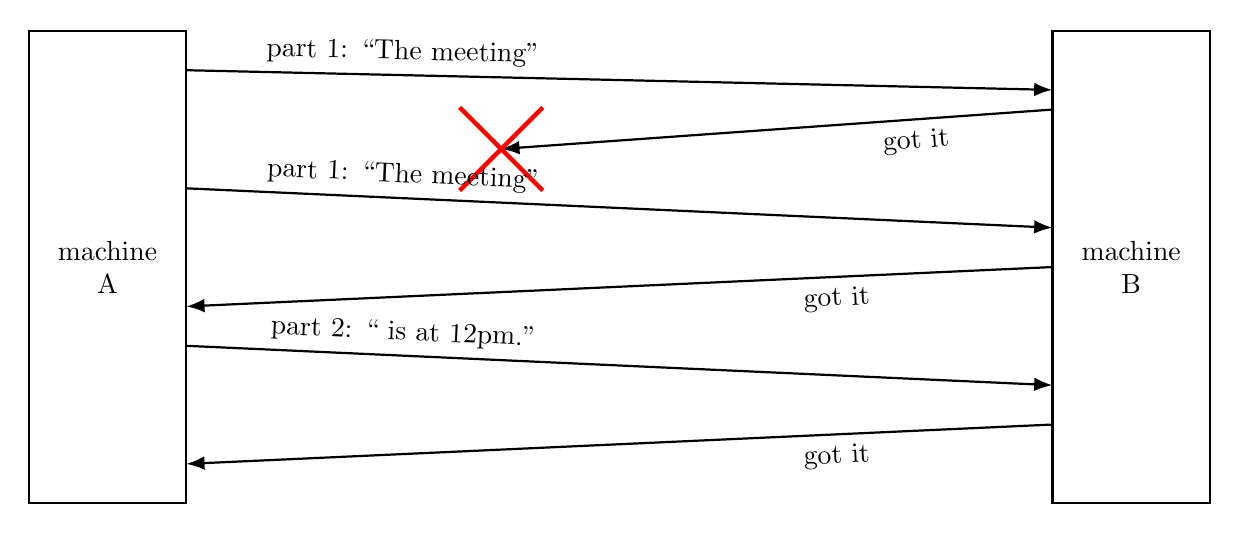
\begin{tikzpicture}
\tikzset{
    box/.style={thick},
    message/.style={draw,thick,-Latex},
    failure/.style={draw,ultra thick,red,cross out,minimum width=1cm,minimum height=1cm},
}
\begin{scope}
\draw[box] (0, 0) rectangle ++(2, -6) 
    node[midway,align=center] {machine\\A};
\draw[box] (13, 0) rectangle ++(2, -6) 
    node[midway,align=center] {machine\\B};
\draw[message] (2, -0.5) -- (13, -0.75) node[pos=0.25, above, sloped] {part 1: ``The meeting''};
\draw[message] (13, -1) -- (6, -1.5) node[pos=0.25, sloped,below] {got it} node[failure] {};
\draw[message] (2, -2) -- (13, -2.5) node[pos=0.25, above, sloped] {part 1: ``The meeting''};
\draw[message] (13, -3) -- (2, -3.5) node[pos=0.25, sloped,below] {got it};
\draw[message] (2, -4) -- (13, -4.5) node[pos=0.25, above, sloped] {part 2: `` is at 12pm.''};
\draw[message] (13, -5) -- (2, -5.5) node[pos=0.25, sloped,below] {got it};
\end{scope}
\end{tikzpicture}
reconstructed message: \\
The meeting is at 12pm.
\end{frame}

\begin{frame}{splitting messages: try 2 --- problem}
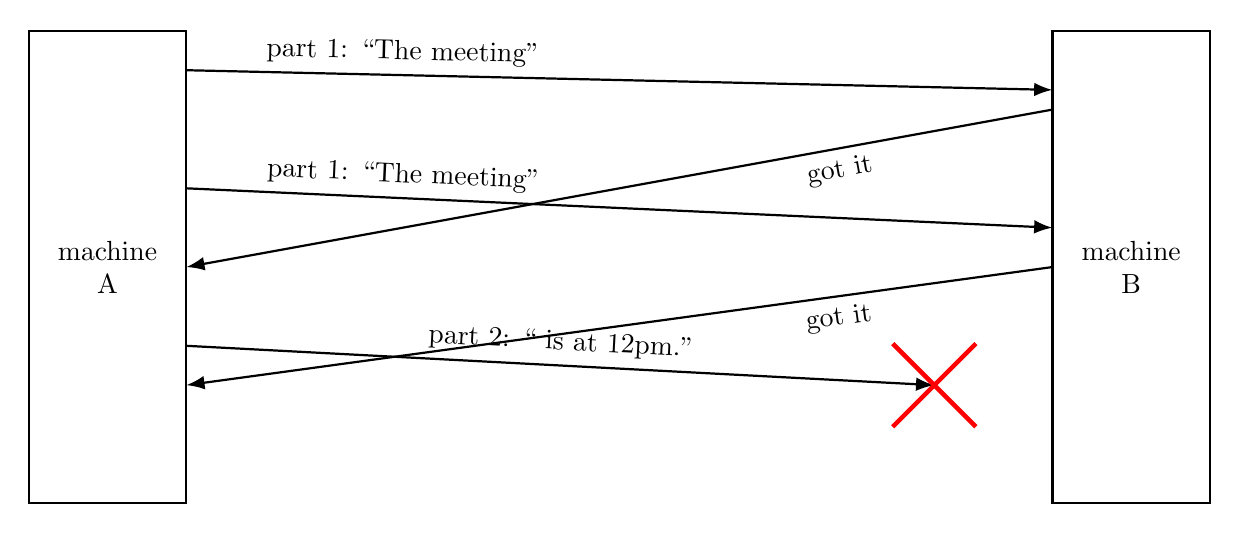
\begin{tikzpicture}
\tikzset{
    box/.style={thick},
    message/.style={draw,thick,-Latex},
    failure/.style={draw,ultra thick,red,cross out,minimum width=1cm,minimum height=1cm},
}
\begin{scope}
\draw[box] (0, 0) rectangle ++(2, -6) 
    node[midway,align=center] {machine\\A};
\draw[box] (13, 0) rectangle ++(2, -6) 
    node[midway,align=center] {machine\\B};
\draw[message] (2, -0.5) -- (13, -0.75) node[pos=0.25, above, sloped] {part 1: ``The meeting''};
\draw[message] (13, -1) -- (2, -3) node[pos=0.25, sloped,below] {got it};
\draw[message] (2, -2) -- (13, -2.5) node[pos=0.25, above, sloped] {part 1: ``The meeting''};
\draw[message] (13, -3) -- (2, -4.5) node[pos=0.25, sloped,below] {got it};
\draw[message] (2, -4) -- (11.5, -4.5) node[pos=0.5, above, sloped] {part 2: `` is at 12pm.''}
    node[failure] {};
\end{scope}
\end{tikzpicture}
A thinks: part 1 + part 2 acknowleged!
\end{frame}

\begin{frame}{splitting messages: version 3}
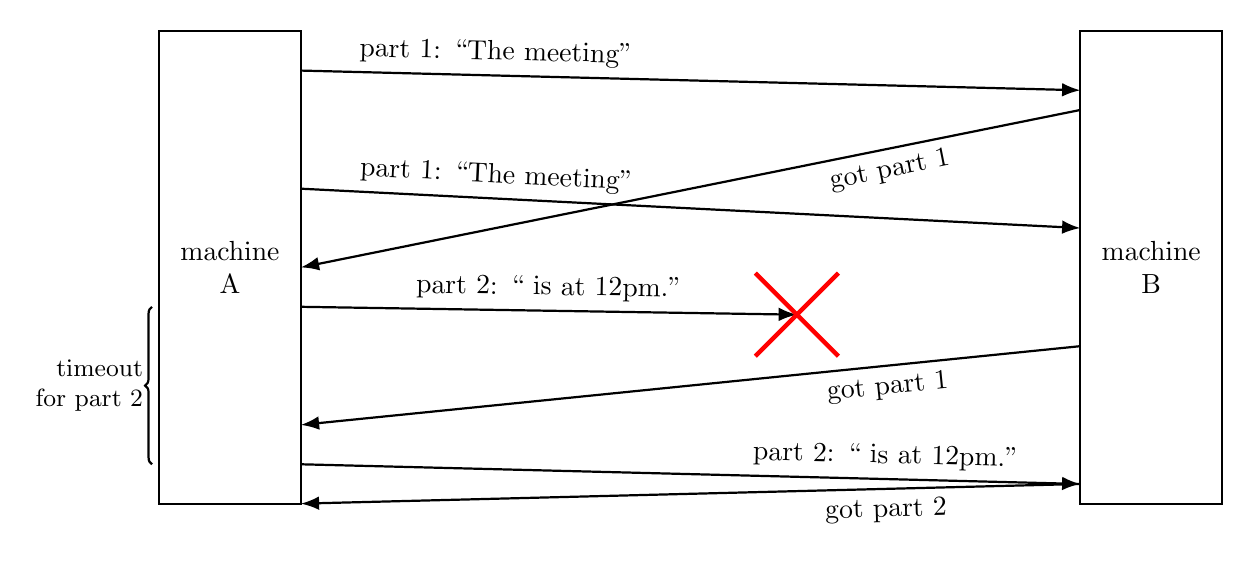
\begin{tikzpicture}
\tikzset{
    box/.style={thick},
    message/.style={draw,thick,-Latex},
    failure/.style={draw,ultra thick,red,cross out,minimum width=1cm,minimum height=1cm},
}
\begin{scope}[xshift=1cm,x=0.9cm]
\draw[box] (0, 0) rectangle ++(2, -6) 
    node[midway,align=center] {machine\\A};
\draw[box] (13, 0) rectangle ++(2, -6) 
    node[midway,align=center] {machine\\B};
\draw[message] (2, -0.5) -- (13, -0.75) node[pos=0.25, above, sloped] {part 1: ``The meeting''};
\draw[message] (13, -1) -- (2, -3) node[pos=0.25, sloped,below] {got \myemph{part 1}};
\draw[message] (2, -2) -- (13, -2.5) node[pos=0.25, above, sloped] {part 1: ``The meeting''};
\draw[message] (13, -4) -- (2, -5) node[pos=0.25, sloped,below] {got \myemph{part 1}};
\draw[message] (2, -3.5) -- (9, -3.6) node[pos=0.5, above, sloped] {part 2: `` is at 12pm.''}
    node[failure] {};
\draw[thick,decorate,decoration={brace,mirror}] (-0.1, -3.5) -- (-0.1, -5.5) node[inner sep=1mm,font=\small,align=right,midway,left] {timeout\\\myemph{for part 2}};
\draw[message] (2, -5.5) -- (13, -5.75) node[pos=0.75, above, sloped] {part 2: `` is at 12pm.''};
\draw[message] (13, -5.75) -- (2, -6) node[pos=0.25, below, sloped] {got \myemph{part 2}};
\end{scope}
\end{tikzpicture}
\end{frame}
